\documentclass{article}
\usepackage{amsmath}
\usepackage{amssymb}
\usepackage{graphicx}
\usepackage{hyperref}
\usepackage[version=4]{mhchem}


\begin{document}
\(B\) is the trisection point of the side \(A C\) of \(\triangle A F C\). Draw a line through \(B\) to meet the extension of \(C F\) at \(E\), to meet \(A F\) at \(D\) such that \(\frac{E D}{D B}=\frac{A B}{B C}=\frac{2}{1}\). Show that \(\frac{A D}{D F}=\frac{7}{2}\).

Solution:
\begin{center}
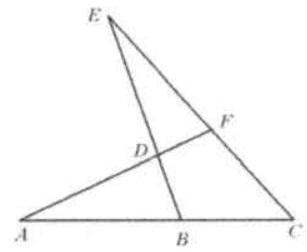
\includegraphics[width=\textwidth]{images/111(3).jpg}
\end{center}

Method 1:\\
As shown in the figure to the right, draw \(D G / / A G\) through \(D\) to meet \(E C\) at \(G\).

In \(\triangle F A C, \frac{F A}{F D}=\frac{A C}{D G}=\frac{3 B C}{D G}\)\\
\centering
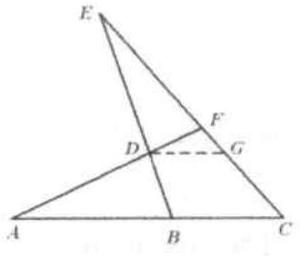
\includegraphics[width=\textwidth]{images/111(2).jpg}

In \(\triangle E B C, \frac{B C}{D G}=\frac{E B}{E D}=\frac{3}{2}\)\\
Substituting (2) into (1) gives us: \(\frac{A F}{F D}=\frac{9}{2} \Rightarrow \frac{A D}{D F}=\frac{7}{2}\)

Method 2:\\
As shown in the figure to the right, draw \(D G / / C E\) through \(D\) to meet \(A C\) at \(G\).\\
In \(\triangle B E C, \frac{B G}{G C}=\frac{B D}{D E}=\frac{1}{2} \quad \Rightarrow \quad \frac{B C}{G C}=\frac{3}{2}\)\\
\centering
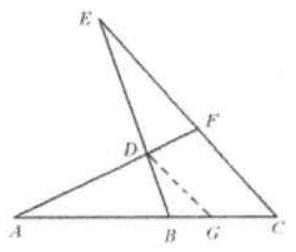
\includegraphics[width=\textwidth]{images/111(1).jpg}


Since \(B C=\frac{1}{3} A C, \frac{A C}{G C}=\frac{9}{2}\)\\
In \(\triangle A C F, \frac{A F}{D F}=\frac{A C}{G C}, \therefore \frac{A F}{D F}=\frac{9}{2}, \therefore \frac{A D}{D F}=\frac{7}{2}\).\\
Method 3:\\
As shown in the figure to the right, draw \(B G / / A F\) through \(B\) to meet \(C E\) at \(G\).\\
In \(\triangle C F A, \frac{A F}{B G}=\frac{A C}{B C}=\frac{3}{1}\),\\
In \(\triangle E B G, \frac{B G}{D F}=\frac{E B}{E D}=\frac{3}{2}\),\\
\centering
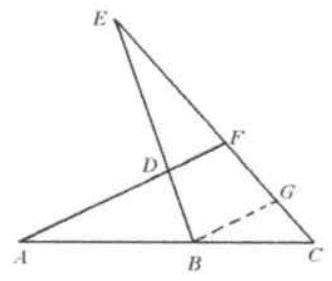
\includegraphics[width=\textwidth]{images/112(1).jpg}\\
(1) \(\times\) (2): \(\frac{A F}{D F}=\frac{9}{2}, \quad \therefore \frac{A D}{D F}=\frac{7}{2}\).

Method 4:\\
As shown in the figure to the right, draw \(B G / / C E\) through \(B\) to meet \(A F\) at \(G\).\\
Since \(\triangle E F D \sim \triangle B G D, \frac{D F}{D G}=\frac{E D}{D B}=\frac{2}{1}\).\\
Therefore \(D G=\frac{1}{2} D F\)\\
In \(\triangle A C F, \frac{A G}{A F}=\frac{A B}{A C}=\frac{2}{3}\). In other words,\\
\centering
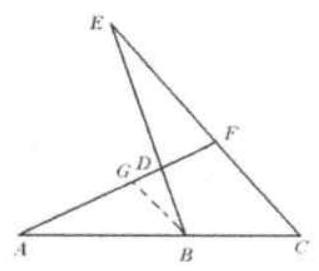
\includegraphics[width=\textwidth]{images/112.jpg}\\
\(\frac{A D-D G}{A D+D F}=\frac{2}{3} . \quad \frac{A D-\frac{1}{2} D F}{A D+D F}=\frac{2}{3}\).\\
Simplifying yields: \(\frac{A D}{D F}=\frac{7}{2}\).\\
Method 5:\\
As shown in the figure to the right, draw \(A G / / C E\) through \(A\) to meet the extension of \(C E\) at \(G\).\\
In \(\triangle A C G, \frac{B E}{A G}=\frac{B C}{A C}=\frac{1}{3}\)


In \(\triangle A F G, \frac{A G}{D E}=\frac{A F}{D F}\)\\
(1) \(\times\) (2): \(\frac{B E}{D E}=\frac{A F}{3 D F}\)

Since \(\frac{B E}{D E}=\frac{3}{2}, \frac{3}{2}=\frac{A F}{3 D F}, \frac{A F}{D F}=\frac{9}{2}\).\\
Hence \(\frac{A D}{D F}=\frac{7}{2}\).\\
\centering
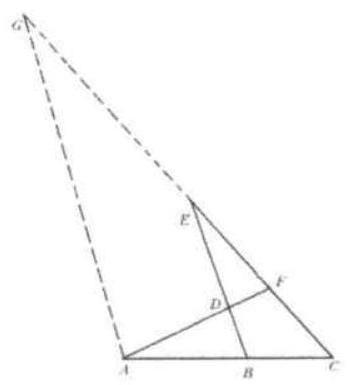
\includegraphics[width=\textwidth]{images/113.jpg}

Method 6:\\
As shown in the figure to the right, draw \(A G / / C E\) through \(A\) to meet the extension of \(E B\) at \(G\).

Since \(\triangle A B G \sim \triangle C B E, \frac{B G}{B E}=\frac{A B}{B C}=\frac{2}{1}\) and \(B G=2 E B\)\\
Since \(\triangle F E D \sim \triangle A G D\),\\
\(\frac{D F}{A D}=\frac{E D}{D G}=\frac{E D}{D B+B G}\)\\
\(=\frac{E D}{D B+2 E B}=\frac{2 D B}{D B+6 D B}=\frac{2}{7}\).\\
Therefore \(\frac{A D}{D F}=\frac{7}{2}\).\\
\centering
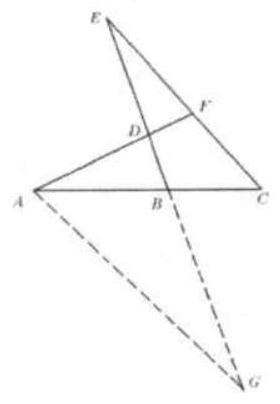
\includegraphics[width=\textwidth]{images/113(2).jpg}

Method 7:\\
As shown in the figure to the right, draw \(E G / / F A\) through \(E\) to meet the extension of \(C A\) at \(G\).\\
In \(\triangle B E G: \frac{E G}{A D}=\frac{E B}{D B}=\frac{G B}{A B}=\frac{3}{1}\)\\
\centering
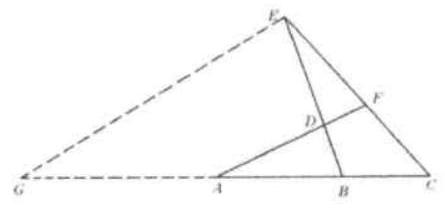
\includegraphics[width=\textwidth]{images/113(1).jpg}

Therefore we have:\\
\(G B=3 A B\)\\
\(E G=3 A D\)


In \(\triangle C E G\) :\\
\(\frac{E G}{A F}=\frac{G C}{A C}=\frac{G B+B C}{A B+B C}=\frac{3(2 B C)+B C}{2 B C+B C}=\frac{7}{3}\)\\
\(\Rightarrow \quad E G=\frac{7}{3} A F=\frac{7}{3}(A D+D F)\)\\
Substituting (2) into (3): \(3 A D=\frac{7}{3}(A D+D F) \quad \Rightarrow \quad 9 A D=7(A D+D F)\)\\
Therefore \(\frac{A D}{D F}=\frac{7}{2}\).

Method 8:\\
As shown in the figure to the right, draw \(E G / / A B\) through \(E\) to meet the extension of \(A F\) at \(G\).\\
Since \(\triangle D A B \sim \triangle D G E, \frac{E G}{A B}=\frac{E D}{D B}=\frac{D G}{A D}=\frac{2}{1}\).

We have \(E G=2 A B\)\\
\(D G=2 A D\)\\
\centering
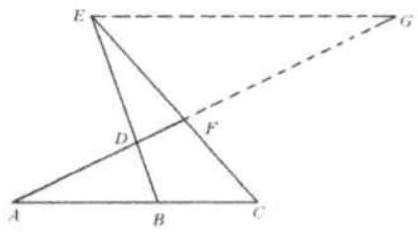
\includegraphics[width=\textwidth]{images/114.jpg}

Since \(\triangle F A C \sim \triangle F G E: \frac{E G}{A C}=\frac{F G}{A F}=\frac{2 A B}{A B+B C}=\frac{2 A B}{A B+\frac{1}{2} A B}=\frac{4}{3}\).\\
We have \(3 F G=4 A F\)\\
Or \(3(D G-D F)=4(A D+D F)\)\\
Substituting (2) into (4):\\
\(3(2 A D-D F)=4(A D+D F) \Rightarrow\)\\
\(6 A D-3 D F=4 A D+4 D F \quad \Rightarrow \quad 2 A D=7 D F\)\\
Therefore \(\frac{A D}{D F}=\frac{7}{2}\).



\end{document}
